\begin{surferPage}[99개의 특이점]{$99$개 특이점을 가지는 $7$차식}
    Oliver Labs은 $2004$년도에 마인츠 대학교에서 졸업논문을 연구하다가 이 $7$차식을 만들었습니다. 이는 아직도 세계기록입니다. 그러나 $104$개의 특이점을 갖는 $7$차식이 존재할지도 모른다고 합니다! Labs의 이 곡면은 칠각형의 대칭성을 가지고 있습니다.(아래 왼쪽 그림 참조) 이 곡면을 위에서 바라보면 더욱 극명해집니다(아래 오른쪽 그림 참조). 

    \vspace*{-0.3em}
    \begin{center}
      \begin{tabular}{c@{\qquad}c}
        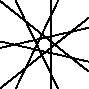
\includegraphics[height=1.5cm]{./../../common/images/labsseptic1.pdf}
        &
        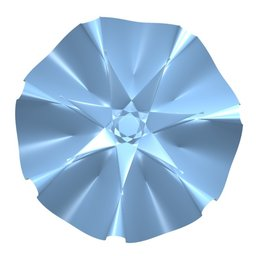
\includegraphics[height=1.5cm]{./../../common/images/labs_septic_von_oben}
      \end{tabular}
    \end{center}
    \vspace*{-0.3em}

이 곡면을 만들어내기 위해 Oliver Labs는 독일의 카이져슬라우테른 대학에서 개발한 {\sc Singular} 라는 소프트웨어를 사용하였습니다. 이 프로그램은 계산 대수기하와 특이점 계산에 최적화 되어있습니다. 

그는 시계처럼 유한한 집합 내의 계산을 이용하였습니다. 예를 들면 24.00$=$0.00, 24.00 $+$ 1 시간은 25.00시가 아닙니다. 1.00시인 것 처럼요.
\end{surferPage}
